\documentclass{article}
\usepackage{graphicx}
\usepackage{amsmath}
\usepackage{pgfplots}
\usepackage[margin=1.5cm]{geometry}
\usepackage{adjustbox}
\usepackage{hyperref}
\usepackage{cite}
\usepackage{listings}
\usepackage{xcolor}
\usepackage{comment}
\usepackage{graphicx}
\usepackage{pdfpages}
\usepackage{enumitem}
\usepackage{pgfplotstable}
\usepackage{booktabs}
\usepackage{adjustbox}
\usepackage{changepage}
\usepackage[utf8]{inputenc}
\lstset{ 
literate= {á}{{\'a}}1 
    {é}{{\'e}}1 
    {í}{{\'i}}1 
    {ó}{{\'o}}1 
    {ú}{{\'u}}1
} 

\hypersetup{
colorlinks=true,
linkcolor=blue,
urlcolor=blue,
}

\pgfplotsset{compat=1.17}
\usepackage[portuguese]{babel}

\definecolor{codegreen}{rgb}{0,0.6,0}
\definecolor{codegray}{rgb}{0.5,0.5,0.5}
\definecolor{codepurple}{rgb}{0.58,0,0.82}
\definecolor{backcolour}{rgb}{0.95,0.95,0.92}

\lstdefinestyle{mystyle}{
    backgroundcolor=\color{backcolour},   
    commentstyle=\color{codegreen},
    keywordstyle=\color{magenta},
    numberstyle=\tiny\color{codegray},
    stringstyle=\color{codepurple},
    basicstyle=\ttfamily\footnotesize,
    breakatwhitespace=false,         
    breaklines=true,                 
    captionpos=b,                    
    keepspaces=true,                 
    numbers=left,                    
    numbersep=5pt,                  
    showspaces=false,                
    showstringspaces=false,
    showtabs=false,                  
    tabsize=2
}

\lstset{style=mystyle}

\title{APS 02 - Estudo de Caso: Indústria 4.0}
\author{Gabriel de Paula Gaspar Pinto}
\date{}

\begin{document}

\maketitle

\paragraph{} O artigo selecionado foi o "Using Machine Learning for Non-Functional Requirements Classification: A Practical Study", dos anais do III Workshop Brasileiro de Engenharia de Software Inteligente, da SBC Open Lib, \href{https://sol.sbc.org.br/index.php/ise/article/view/26121/25944}{disponível aqui}.

% exercicio 1
\section{Quais foram os requisitos funcionais e não funcionais considerados no desenvolvimento do sistema inteligente descrito no estudo?}

\paragraph{} No estudo conduzido pelos autores, foi utilizada a base de dados PROMISE, que contém especificações de requisitos de software divididas entre funcionais e não funcionais. Embora estejam presentes, os requisitos funcionais não foram o foco da análise. Eles representaram aproximadamente 255 requisitos funcionais, que se referem às funcionalidads esperadas de um sistema, conforme descrito pelas partes interessadas (stakeholders). 
\paragraph{} Por outro lado, os requisitos não funcionais foram o objeto central do estudo, totalizando 370 requisitos não funcionais, nos quais foram classificados de acordo com a norma ISO/IEC 25010. Entre as categorias estavam disponibilidade, legalidade, aparência, manutenibilidade, operacionalidade, desempenho, escalabilidade, segurança, usabilidade, tolerância à falhas e portabilidade. Esses requisitos foram analisados e classificados de forma automática, através de técnicas de aprendizado de máquina, buscando identificar suas categorias específicas com precisão e eficiência.

% exercicio 2
\section{Modelar uma parte do sistema usando pelo menos um diagrama UML (caso de uso, classes ou atividades)}

\paragraph{} Dado o contexto do artigo, o melhor diagrama a se fazer é o de caso de uso. 

\begin{figure}[ht!]
    \centering
    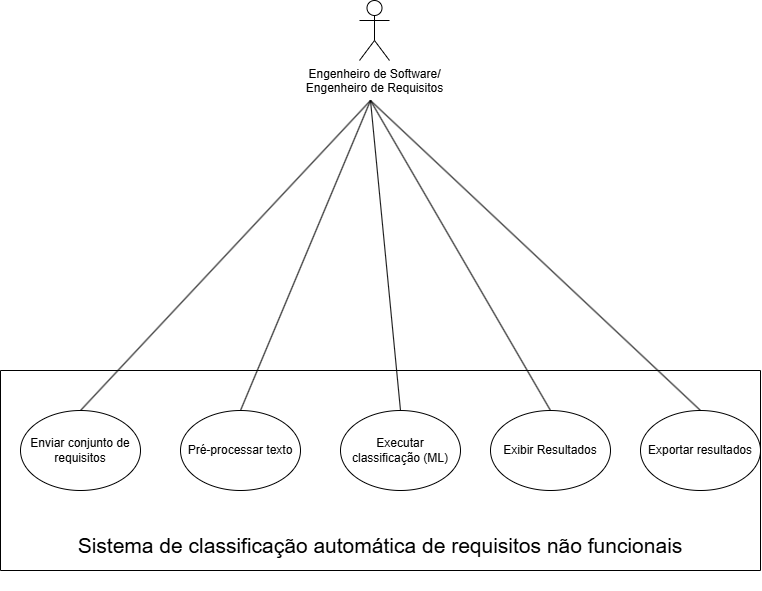
\includegraphics[width=0.5\linewidth]{g.png}
    \caption{Diagrama de caso de uso de um sistema para classificação automática de requisitos não funcionais}
    \label{fig:questao1}
\end{figure}

% exercicio 3
\section{Quais foram os principais desafios técnicos e organizacionais enfrentados na implementação do sistema?} 

\paragraph{} A implementação do sistema inteligente de classificação automática enfrentou diversos desafios, principalmente técnicos. Um dos principais foi o processo de pré-processamento dos dados de texto dos requisitos, que envolveu a remoção de caracteres especiais, padronização de maiúsculas e minúsculas, exclusão de palavras irrelevantes e a tokenização das sentenças, com este último método sendo utilizado em múltiplas inteligências artificiais generativas.
\paragraph{} Outro desafio foi a escolha adequada das técnicas de extração de características e dos algoritmos de aprendizado de máquina mais eficazes. A equipe optou pela técnica TF-IDF (Term Frequency-Inverse Document Frequency) para transformar o texto em representações numéricas e avaliou diversos classificadores, como KNN (K-nearest Neighbors), SVM (Support Vector Machines), árvores de decisão (Dtree) e, especialmente, o algoritmo SGD (Stochastic Gradient Descent), que demonstrou os melhores resultados.
\paragraph{} Além disso, houve a preocupação com possíveis vieses nos dados, já que o dataset utilizado já estava rotulado, e não havia como garantir a total precisão dessas rotulações. Para mitigar tais riscos, os experimentos foram conduzidos com validação cruzada. Embora o estudo não tenha sido realizado diretamente em uma indústria, os autores apontam a necessidade de validar esses resultados em contextos reais, o que representa um desafio importante para que a solução proposta seja aplicável fora do ambiente controlado de pesquisa.

% exercicio 4
\section{De que maneira a introdução da IA afetou os processos de produção e a qualidade dos produtos?}

\paragraph{} Embora o estudo não trate diretamente de um processo de produção industrial tradicional, a introdução da inteligência artificial na classificação de requisitos de software representa um impacto direto na qualidade do desenvolvimento de sistemas. Ao automatizar a identificação de requisitos não funcionais, a proposta reduz o esforço manual e os erros associados à classificação subjetiva, além de acelerar significativamente esse processo.
\paragraph{} Como consequência, os sistemas podem ser projetados levando em consideração desde cedo aspectos importantes, como desempenho, usabilidade e segurança, o que contribui para a entrega de produtos mais robustos, confiáveis e alinhados às expectativas de qualidade, em um período de tempo menor. Por fim, isso pode ajudar a diminuir custos com reparação de requisitos e falhas em fases mais avançadas do desenvolvimento.

% exercico 5
\section{Quais lições podem ser extraídas deste estudo de caso para projetos futuros de sistemas inteligentes?}

\paragraph{} Este estudo oferece lições valiosas para projetos futuros que envolvam sistemas inteligentes, sendo uma das principais a constatação de que a preparação adequada dos dados é fundamental para o sucesso de modelos de aprendizado de máquina. A escolha da técnica TF-IDF, junto com o classificados SGD, mostrou-se altamente eficaz na classificação de requisitos não funcionais, o que sugere que esta combinação pode ser um ponto de partida para aplicações similares. 
\paragraph{} Além disso, o estudo destaca a importância de trabalhar com conjuntos de dados confiáveis e bem rotulados, bem como de aplicar validação cruzada para garantir resultados robustos. Outro ponto importante é a necessidade de levar esses modelos para ambientes reais, fora do laboratório, para validar sua aplicação.
\paragraph{} Por fim, a pesquisa mostra que a integração de inteligências artificiais em processos de engenharia de software pode gerar ganhos significativos, em relação a qualidade e produtividade, desde que seja integrada com critérios técnicos rigorosos e uma visão clara dos objetivos.

\end{document}